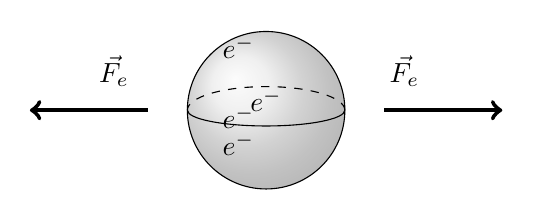
\begin{tikzpicture}
        \shade[ball color = gray!40, opacity = 0.4] (0,0) circle (1cm);
        \draw (0,0) circle (1cm);
        \draw (-1,0) arc (180:360:1 and  0.2);
        \draw[dashed] (1,0) arc (0:180:1 and 0.3);
        \node[left = 10, above = -20]{\(e^-\)};
        \node[left = 0, above = -4]{\(e^-\)};
        \node[left = 10, above = 15]{\(e^-\)};
        \node[left = 10, above = -10]{\(e^-\)};
        \node[right = 50, above = 5]{\(\vec{F_e}\)};
        \draw[->,ultra thick] (1.5,0)--(3,0);
        \node[right = -55, above = 5]{\(\vec{F_e}\)};
        \draw[->,ultra thick] (-1.5,0)--(-3,0);
\end{tikzpicture}